\documentclass{scrartcl}			% defines the kind of document you want to produce

% Include different packages:
\usepackage[utf8]{inputenc}
\usepackage[T1]{fontenc}
\usepackage{lmodern}
\usepackage[english]{babel}
\usepackage{amsmath}
\usepackage{graphicx}           	% include graphics
\usepackage{caption}	
\usepackage{subcaption}	 
\usepackage{hyperref}
\usepackage{epstopdf}
\usepackage{siunitx}
\usepackage{float}

\title{Neuroprothetik Exercise 3 \\ Mathematical Basics 2}
\author{ Laura Bielenberg }
\date{22. Mai 2019}

\begin{document} 					% Document begins here

\maketitle

\section{Solver Implementation}	
Implement the following numerical differential equation solvers as functions in Python or Matlab:
\begin{itemize}
\item Forward (Explicit) Euler
\item Heun
\item Exponential Euler
\end{itemize}
All three solvers have been implemented in Python. Their implementation is given in the file \texttt{solver.py}. To generate the plots execute \texttt{plot\_all.py}.

\section{Solve Functions}		% start a new section 
\label{sec:solve}
Solve the differential equation 
\begin{equation}
	\frac{dV}{dt} = 1 - V - t
	\label{dgl1}
\end{equation}
where $V(t=-4.5) = V_0 = -4$ with the solvers implemented above. Vary the stepsize (1s, 0.5s, 0.1s, 0.012s), plot the results and answer the following tasks:

\begin{enumerate}
\item \textit{Interpret the impact of changing the stepsize:}\\
In figures \ref{fig:forwardEul} to \ref{fig:expo} we can see, that by reducing the stepsize all plots reach similar approximations.\\
Especially when using a first order method, such as the Explicit-Euler, it can be seen that the stepsize has an nonneglectable impact on the approximation error. More precisely, the local error for the Explicit-Euler is proportional to $\Delta t^2$ and the global error is proporional to the $\Delta t$, meaning that by reducing the stepsize to a half the error is halfed, too. The other two methods, Heun and Exponential-Euler show similar step-size dependent global error behavior, where bisection of the stepsize leads to quartering of the global error for the Heun Method and halve the global error for the Exponential-Euler.
\item \textit{Why not use an infinitesimal stepsize?}\\
Using an infinitesimal stepsize would increase the computation time and effort considerably. Suitable approximations can already be obtained using suffitiantly small step-sizes.
\end{enumerate}
\pagebreak
\begin{figure}[H]	
	\centering
	\begin{subfigure}[b]{\textwidth}			%start figure-environment
		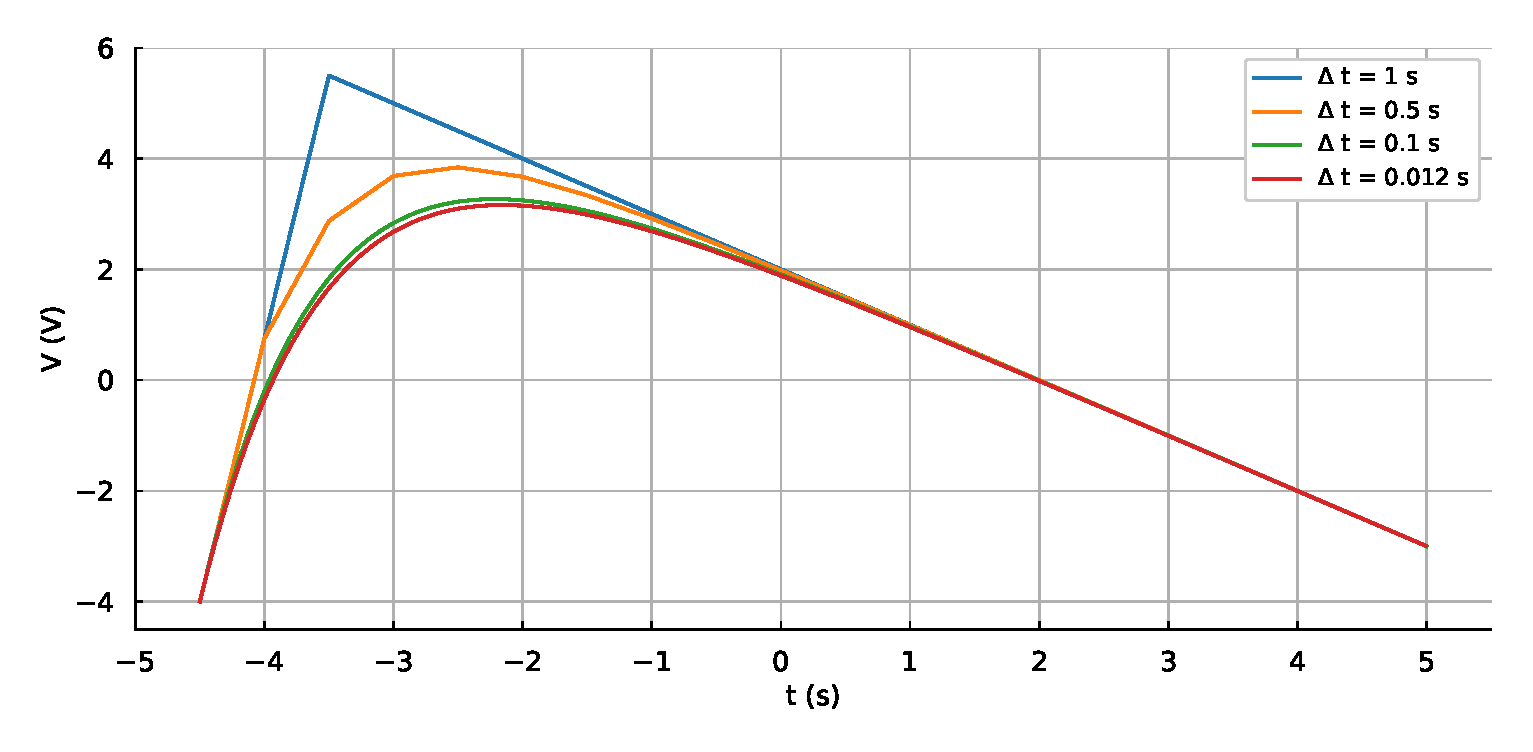
\includegraphics[width=1\linewidth]{imgs/forwardEul.eps}
		\caption{}
		\label{fig:forwardEul} %choose a label, see subsection references
	\end{subfigure}

	\begin{subfigure}[b]{\textwidth}					%start figure-environment
		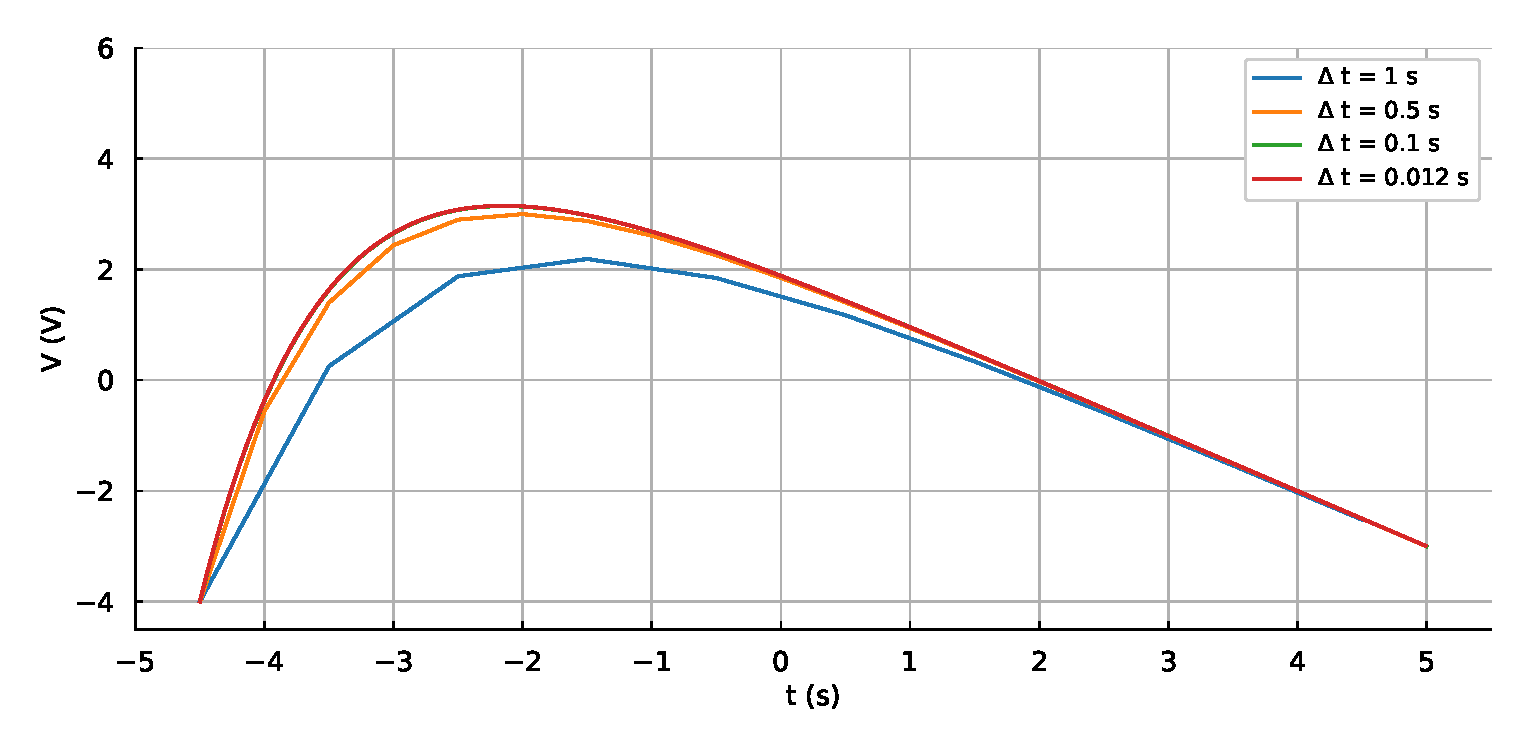
\includegraphics[width=1\linewidth]{imgs/heun.eps}
		\caption{}
		\label{fig:heun} %choose a label, see subsection references
	\end{subfigure}
	
	\begin{subfigure}[b]{\textwidth}					%start figure-environment
		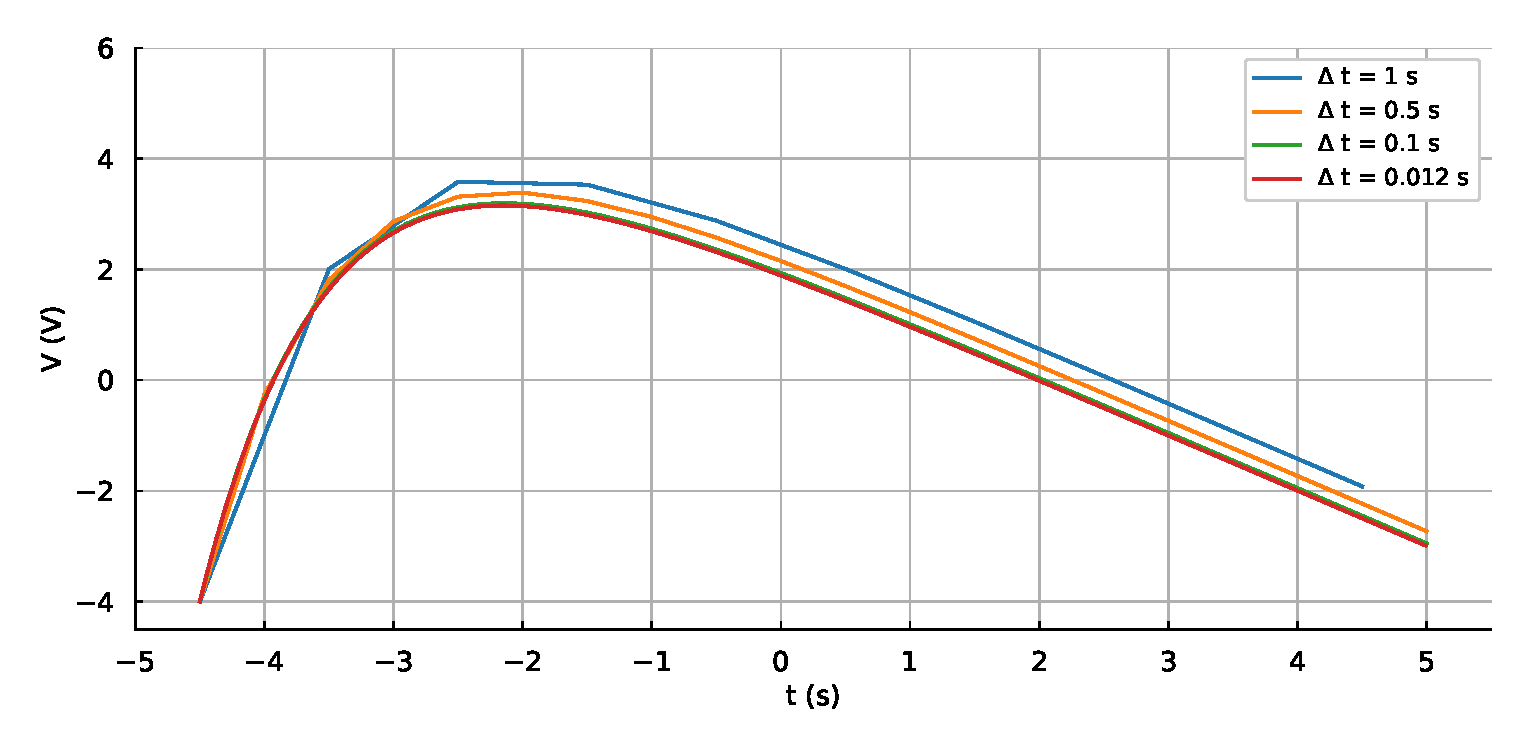
\includegraphics[width=1\linewidth]{imgs/expo.eps}
		\caption{}
		\label{fig:expo} %choose a label, see subsection references
	\end{subfigure}
	\caption{Approximation of the differential equation given in \ref{sec:solve} using different solvers and stepsizes. Figure \ref{fig:forwardEul}: Forward-Euler Method,  figure \ref{fig:heun}: Heun-Method, figure \ref{fig:expo}: Exponential-Euler Method.}
\end{figure}
\pagebreak
\section{The Leaky Integrate and Fire Neuron}
Implement a Leaky Integrate and Fire neuron model according to the following equation:
\begin{equation}
V_{n+1}=\begin{cases}V_n + \frac{\Delta t}{C_m}(-g_{leak}(V_n-V_{rest})+I_{input}(t_n)& V_n < V_{thr}\\V_{spike}&V_{thr} \leq V_n < V_{spike}\\V_{rest}&V_{spike}  \leq V_{n}\end{cases}
\end{equation}
with
\begin{itemize}
\item $V_m$ : cell membrane voltage 
\item $C_m = \SI{1}{\micro\ampere}$ : membrane capacity
\item $g_{leak} = \SI{100}{\micro}$S : leak conductivity
\item $V_{rest} =\SI{-60}{\milli\volt}$ : cell membrane resting voltage
\item $V_{thr} = \SI{-20}{\milli\volt}$ : cell membrane spiking threshold voltage
\item $V_{spike} = \SI{20}{\milli\volt}$ : spiking voltage
\end{itemize}
And simulate $V_n$ for \SI{50}{\micro\second} ($\Delta t = \SI{25}{\micro\second} $) with $I_{input}$ being
\begin{itemize}
\item constant \SI{10}{\micro\ampere}
\item constant \SI{20}{\micro\ampere}
\item rectified 50Hz sine with \SI{10}{\micro\ampere} amplitude
\item rectified 50Hz sine with \SI{30}{\micro\ampere} amplitude
\end{itemize}
Plot and interpret the results.\\
\newline
\textit{Interpretation:}
\newline
In the case of a constant stimulation current $I_{stim}$, as given in figures \ref{fig:10const} and \ref{fig:20const}, it can be seen that the cell membrane voltage increases exponentially, until it hits the threshold $V_{thr}$ at \SI{-20}{\milli\volt}. At that point an action potential is generated where the voltage reaches $V_{spike}$ and is then again reset to the initial resting potential. When comparing \ref{fig:10const} and \ref{fig:20const} we see that, by increasing $I_{stim}$, $V_{stim}$ is reached earlier and thus, since there is no refractory period set for this LIF Neuron model to limit the neuronal firing rate, action potentials are being generated at a higher frequency.
\newline
\newline
When instead setting  $I_{stim}$ to a rectified \SI{50}{\herz}  current, as given in figures \ref{fig:10rect}  and \ref{fig:30rect}, we can see that the voltage increase is not anymore exponential, but depends on the value of  $I_{stim}$ at that point of time. Whenever  $I_{stim}$ reaches zero we can observe a small decline in the otherwise rising slope, probably caused by the leak conductivity. Apart from that, the action potential generation shows the same behaviour as when using a constant current:\\
$V_{m}$ rises $\rightarrow$  $V_{m}$ hits $V_{thr}$ $\rightarrow$ actionpotential is generated $\rightarrow$ reset to initial resting potential.

\begin{figure}[H]	
	\centering
	\begin{subfigure}[b]{\textwidth}			%start figure-environment
	\centering
		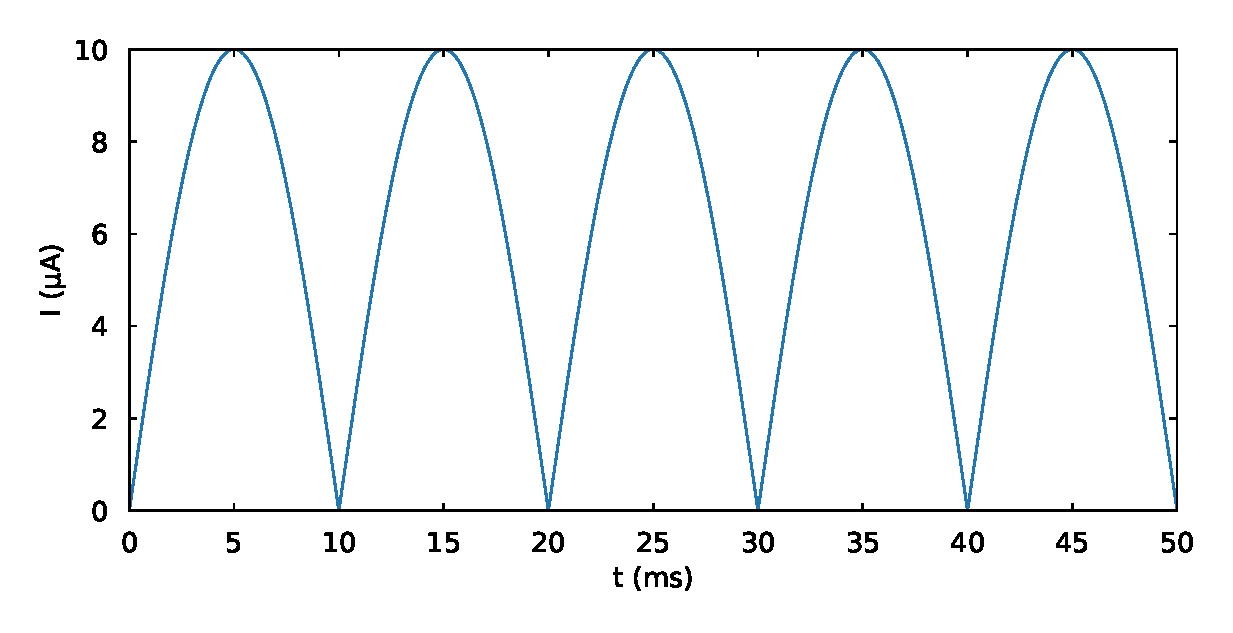
\includegraphics[width=0.8\linewidth]{imgs/1e-05muA_rectSign.eps}
		\caption{Rectified Sine-Input for the LIF model with an amplitude of \SI{10}{\micro\ampere}.}
		\label{fig:10_r} %choose a label, see subsection references
	\end{subfigure}

	\begin{subfigure}[b]{\textwidth}					%start figure-environment
	\centering
		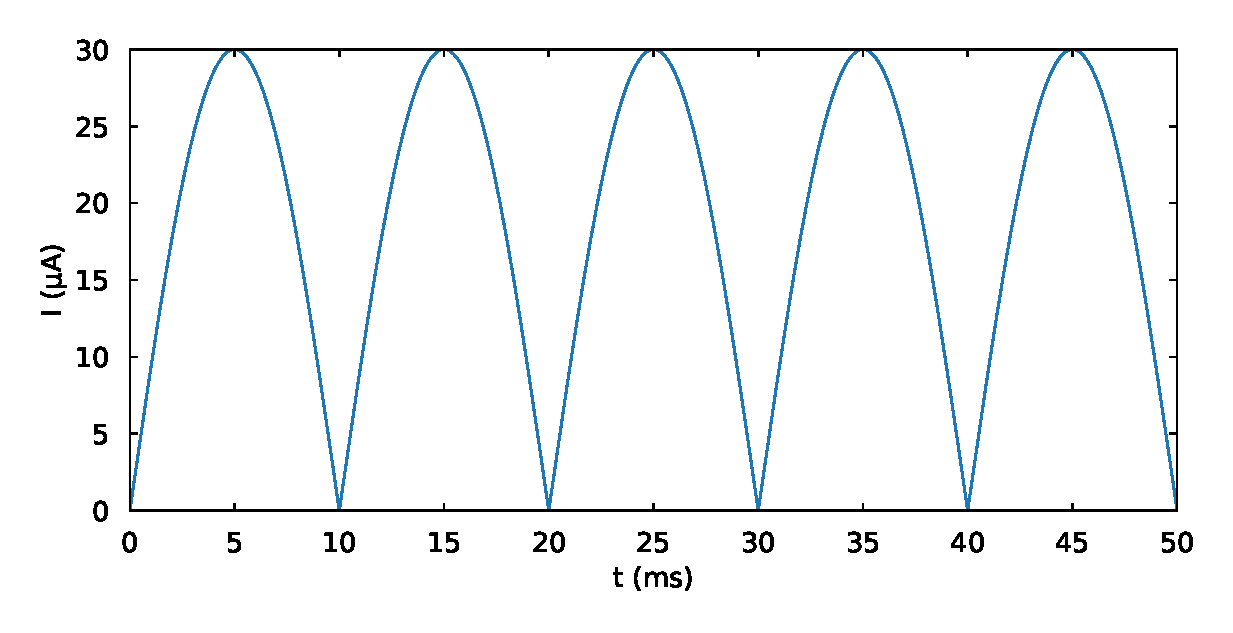
\includegraphics[width=0.8\linewidth]{imgs/3e-05muA_rectSign.eps}
		\caption{Rectified Sine-Input for the LIF model with an amplitude of \SI{30}{\micro\ampere}.}
		\label{fig:30_r} %choose a label, see subsection references
	\end{subfigure}
	\caption{Current inputs for the LIF-Model, outputs visible in figures \ref{fig:10_r} and \ref{fig:30_r} .}
\end{figure}

\begin{figure}[h] 
  \begin{subfigure}[b]{0.5\linewidth}
    \centering
    \includegraphics[width=\linewidth]{imgs/10muA_const_curr.eps} 
    \caption{\SI{10}{\micro\ampere} constant input current.} 
    \label{fig:10const} 
    \quad
  \end{subfigure}%% 
  \begin{subfigure}[b]{0.5\linewidth}
    \centering
    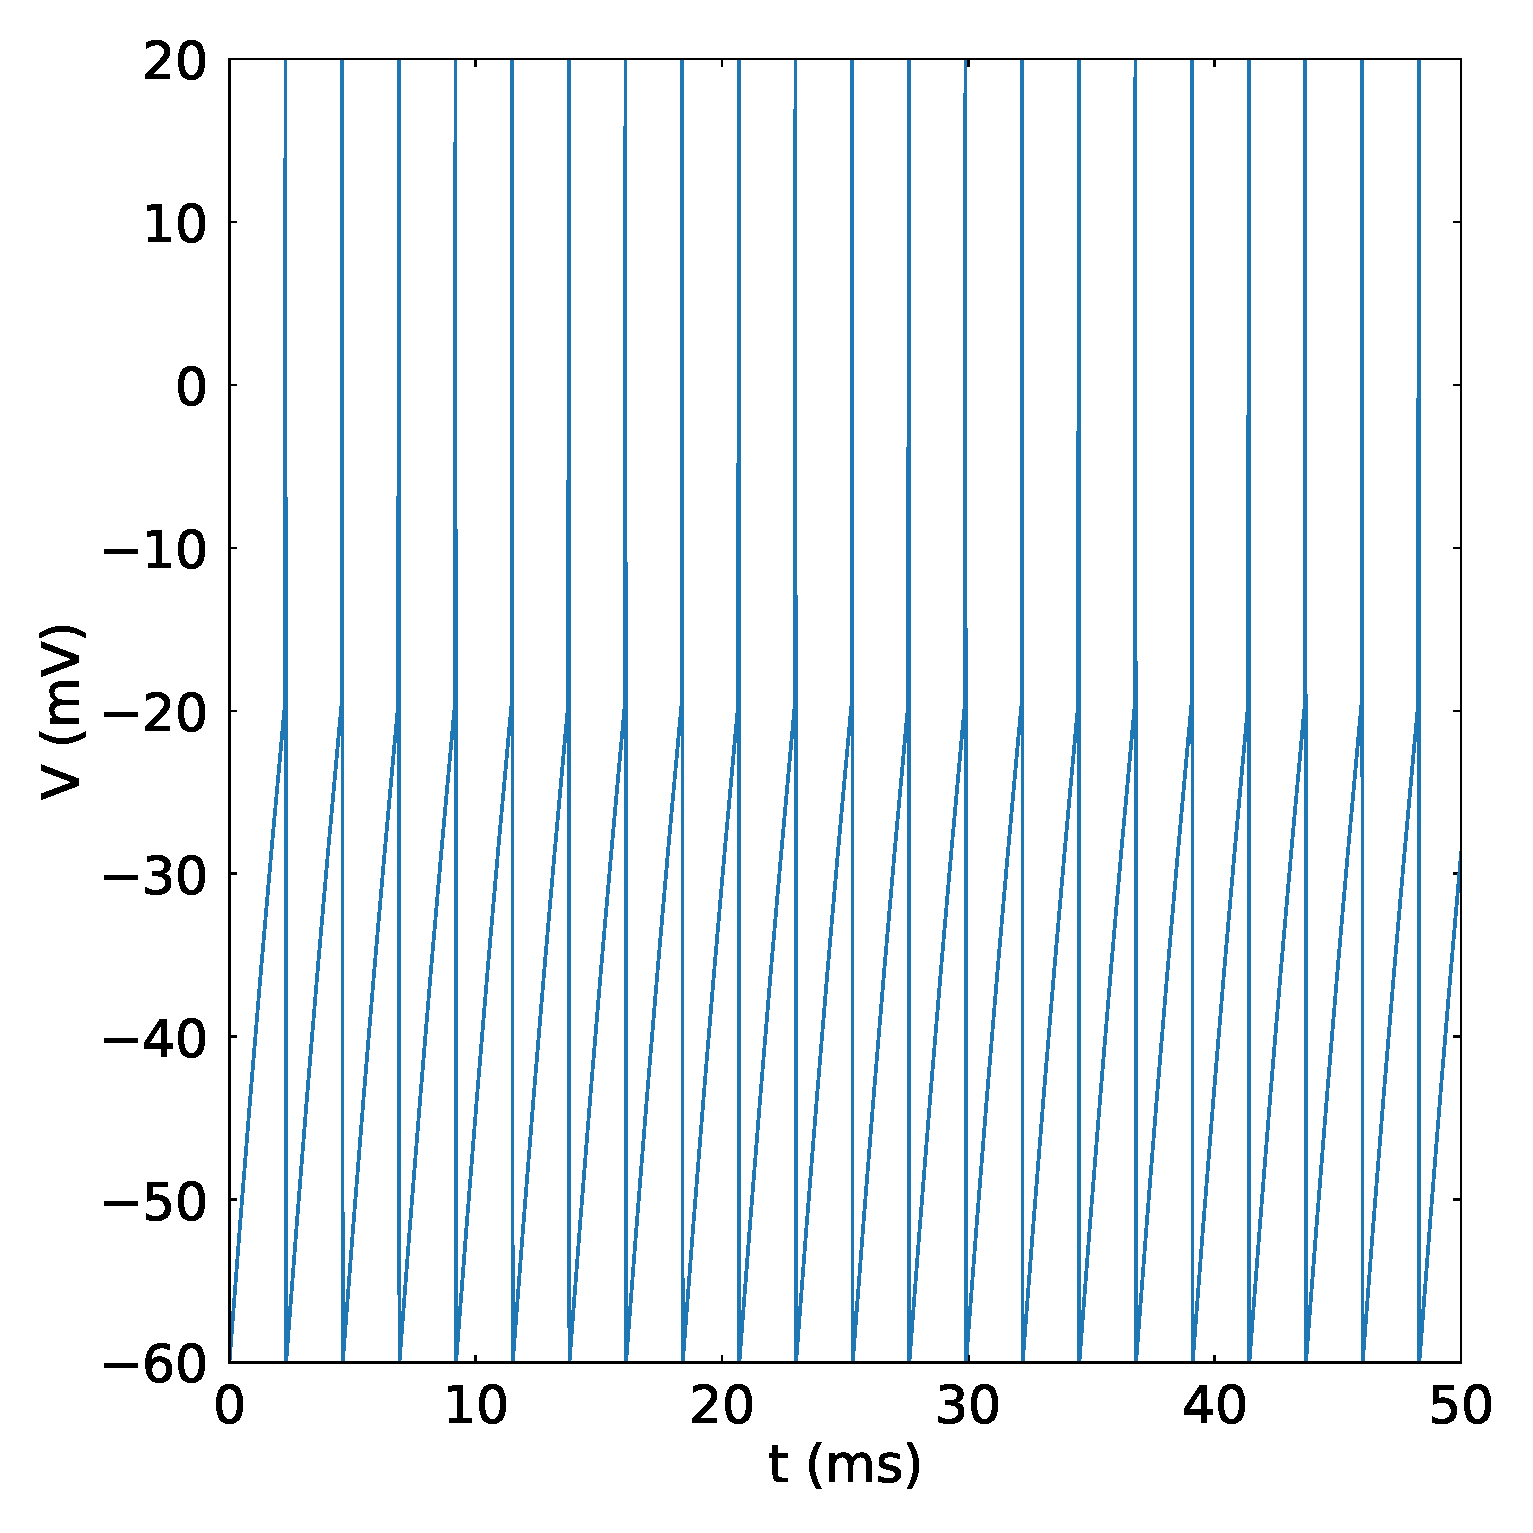
\includegraphics[width=\linewidth]{imgs/20muA_const_curr.eps} 
    \caption{\SI{20}{\micro\ampere} constant input current.} 
    \label{fig:20const} 
    \quad
  \end{subfigure} 
  \begin{subfigure}[b]{0.5\linewidth}
    \centering
    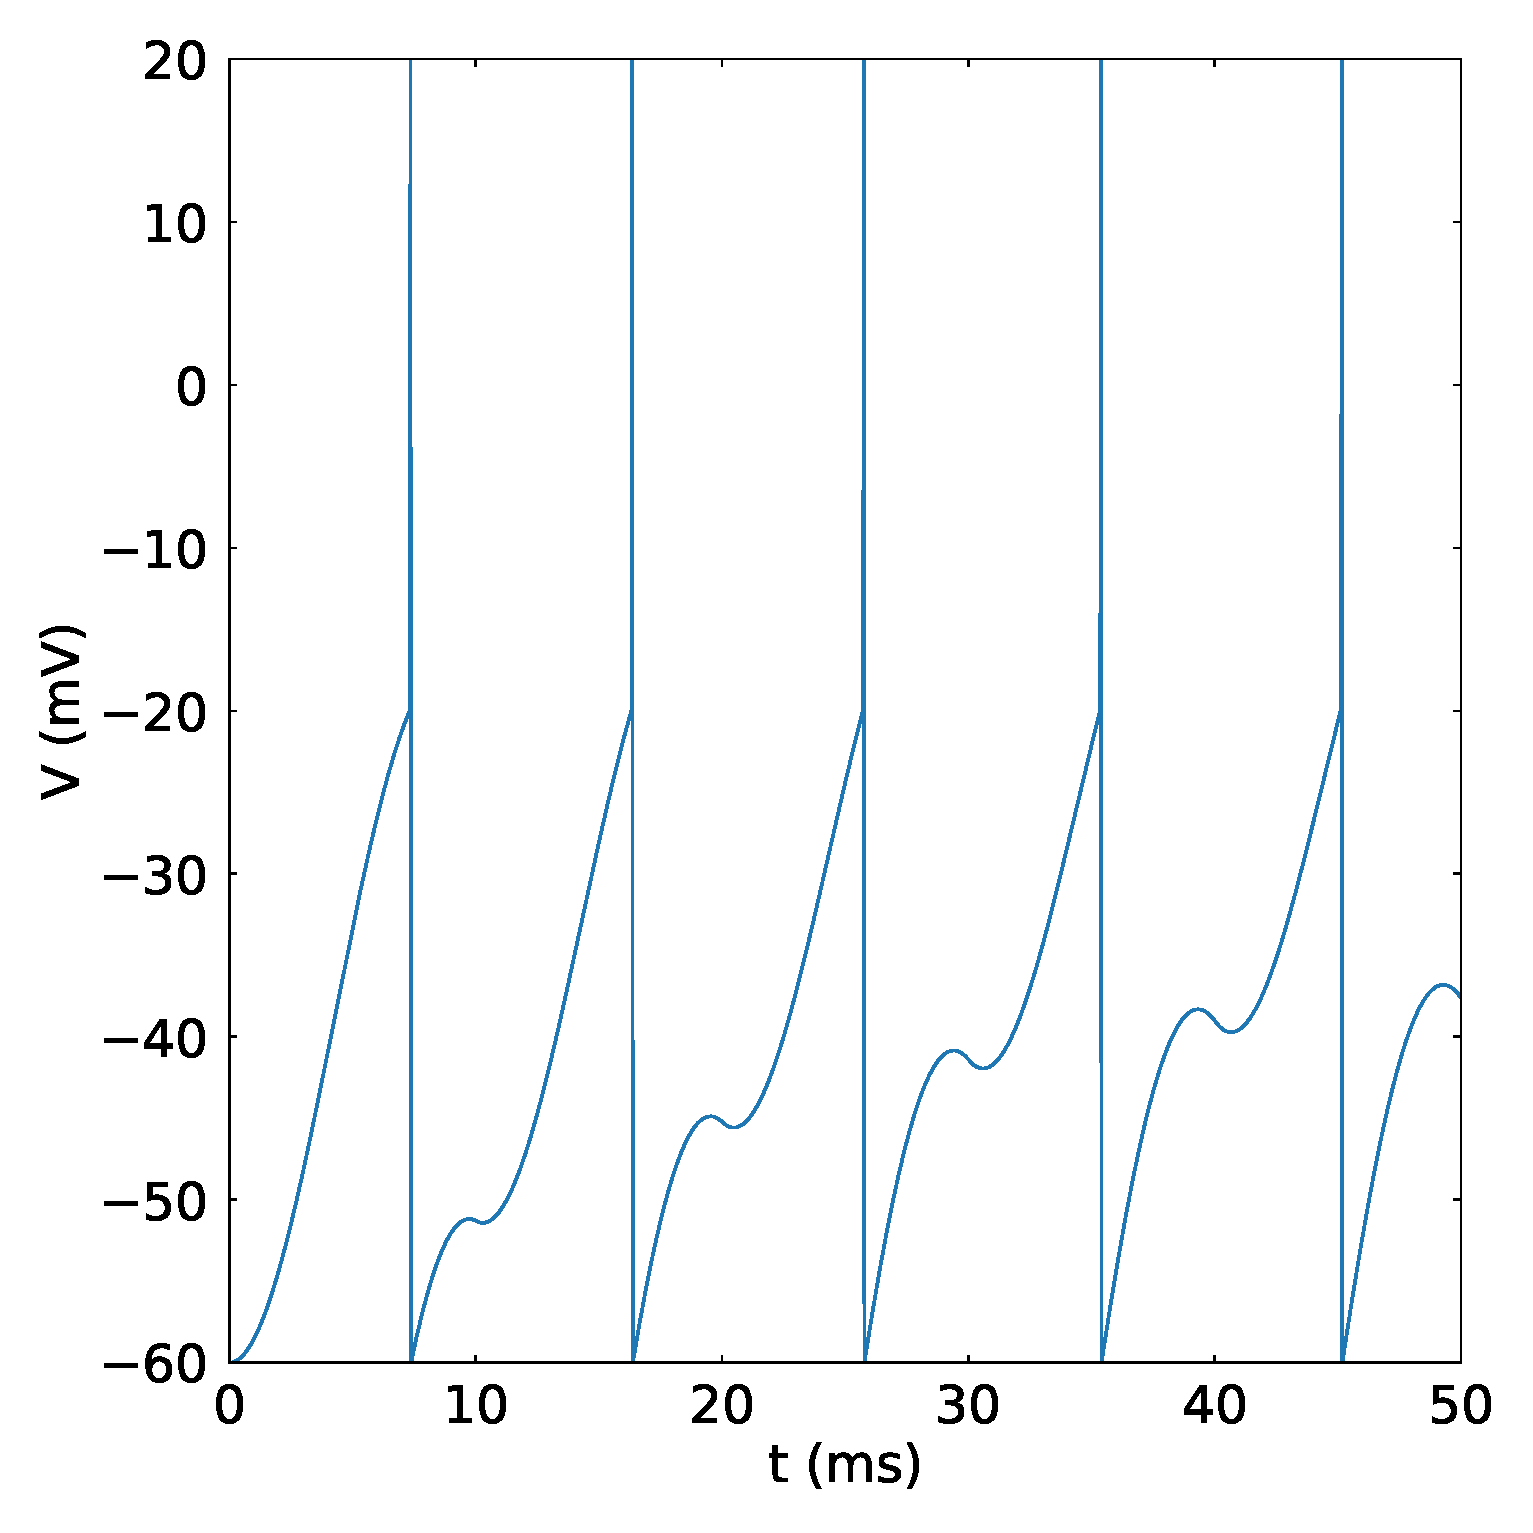
\includegraphics[width=\linewidth]{imgs/10muA_rect_curr.eps} 
    \caption{Rectified input with 50 Hz and \SI{10}{\micro\ampere} amplitude.} 
    \label{fig:10rect} 
  \end{subfigure}%%
  \begin{subfigure}[b]{0.5\linewidth}
    \centering
    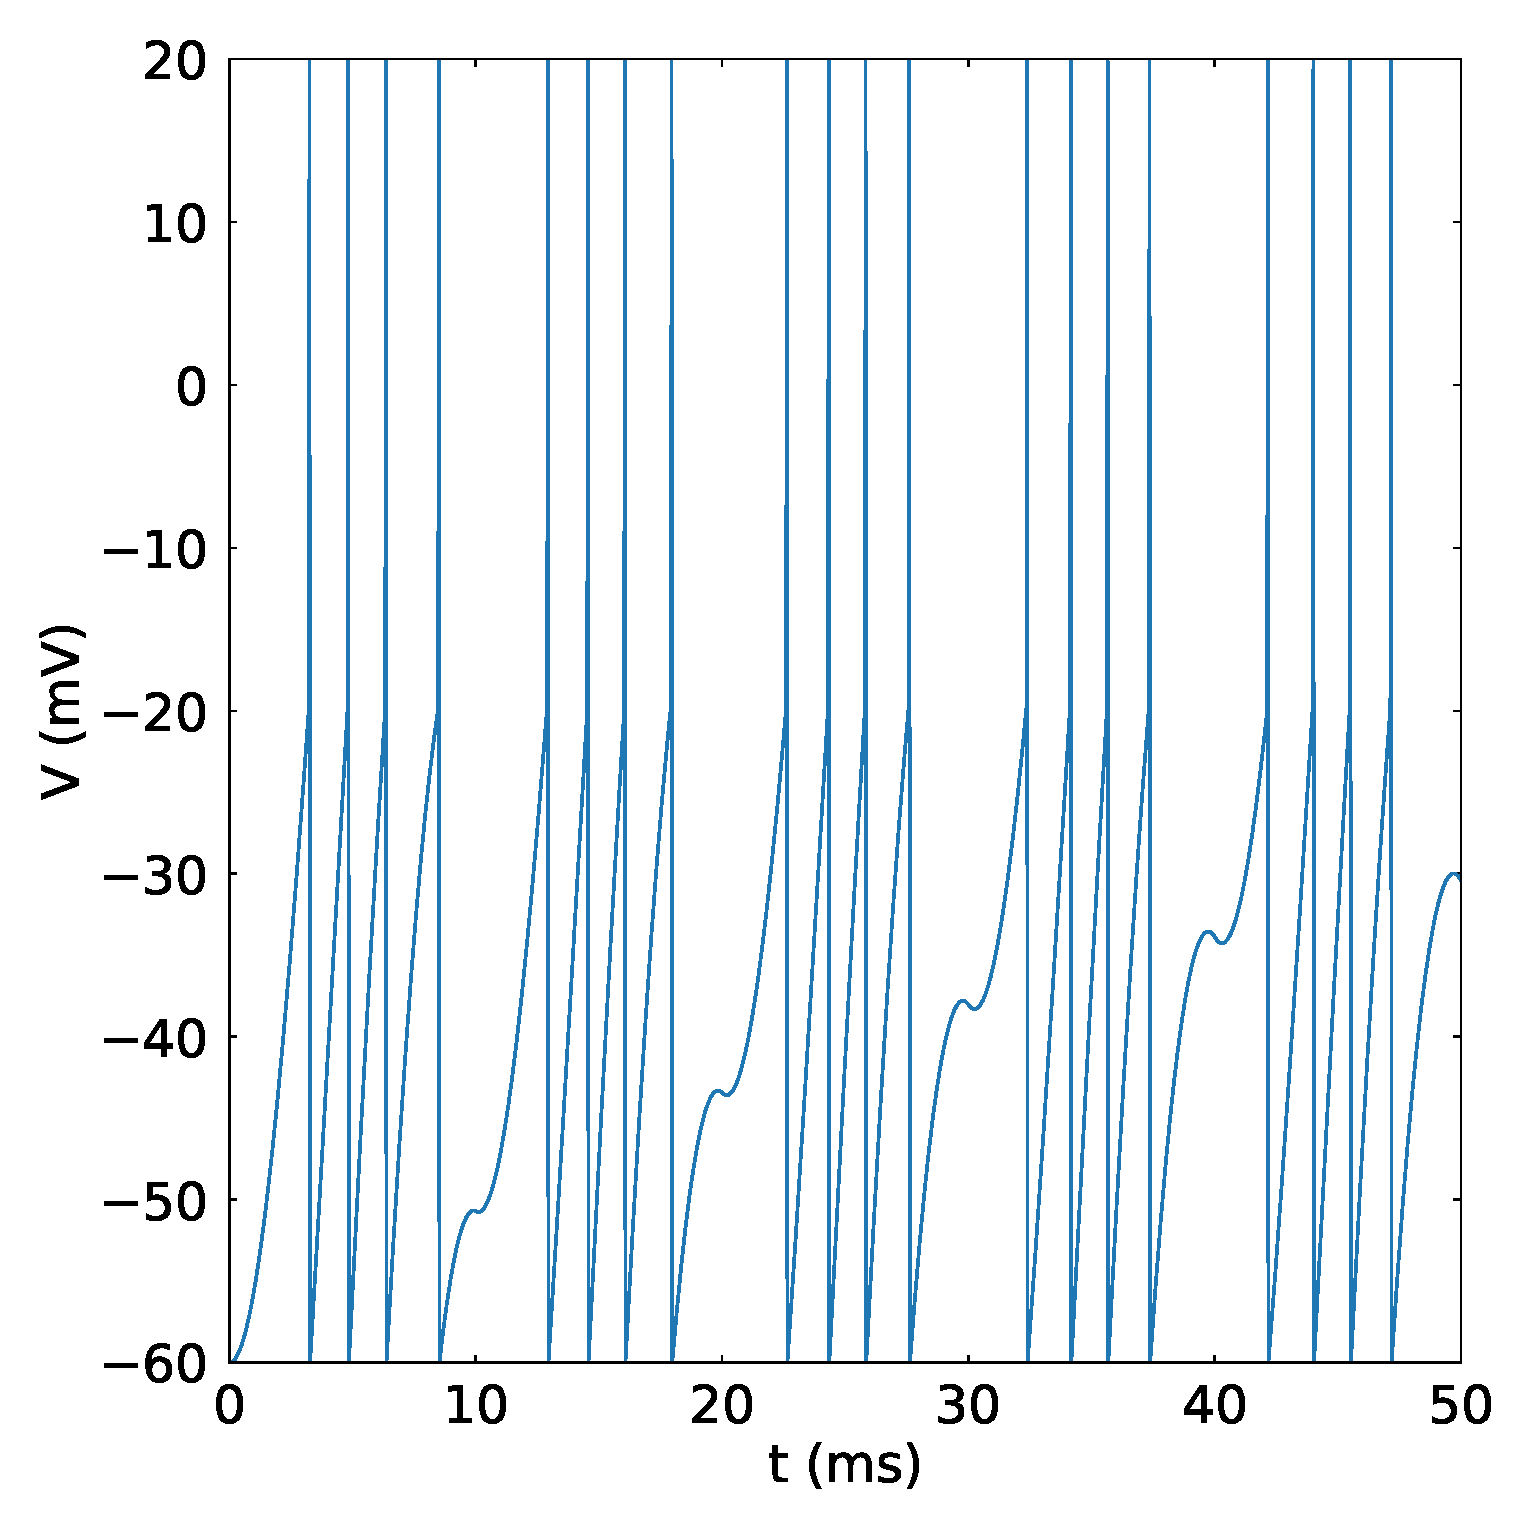
\includegraphics[width=\linewidth]{imgs/30muA_rect_curr.eps} 
    \caption{Rectified input with 50 Hz and \SI{30}{\micro\ampere} amplitude.} 
    \label{fig:30rect} 
    \end{subfigure} 
  \caption{Cell membrane voltage of a LIF-Model using different current inputs.}
  \label{fig:LIF} 
\end{figure}

\end{document}